\section{A thermophysical model for a binary system of asteroids}
\label{mutual}

In this section, we present the implementation of the mutual heating. As Didymos is a binary system of asteroid, the current thermophysical model is not enough to fully describe the temperature at the surface of the asteroid. The Hera mission focuses on the secondary object in this binary system. Its surface temperature depends also on the primary object for two main reasons. 1) the reflection of the Sun on the surface of the primary to the secondary, this phenomenon depends on the primary albedo and on its position with respect to the Sun and the secondary, and it is named the mutual direct heating, 2) the heat received from the primary itself, just as the Sun, considering it as a black body, it only depend on the distance and is called the mutual diffuse heating.

\subsection{Theory}

Didymos’ secondary is modeled in a simplified manner due to the many unknowns and assumptions adopted in this study. This section deals with neglected effects thought to alter surface temperatures in certain cases.

A complete thermophysical model including the direct and diffuse mutual heating is \cite{pelivan}:
\begin{equation}
    Q_{Sun} + W_p + u_p + w_p = \epsilon \sigma u^4 + \kappa \frac{du}{dx},
    \label{eq 41}
\end{equation}
where the direct $Q_{Sun}$ compute from Eq. (\ref{eq 23})\\

For the current simplified model, the mutual heating from Didymain to Didymoon will be small due to the comparatively large distance of 1.18km \cite{Model} between the two bodies and enter through terms $W_p$, $u_p$ and $w_p$. As defined in the reference model, the low albedo allow us to apply the single-scattering mode for which the diffuse thermal heating flux $w_p$ can be neglected. However, this flux will be discussed in the next part.\\

Discretizing the two bodies into facets i for the secondary and j for the primary, the mutual heating from diffuse solar radiation from the primary can be compute using :
\begin{equation}
    W_{p,j} = \sum_{i \neq j}^N V_{ij} \frac{S_{\odot} A cos \varsigma _j (t)}{r^2 (t)} v_{j,sun}.
    \label{eq 42}
\end{equation}
Where $N$ is the total number of facets, $v_{j,sun}$ is the facet view factor to the Sun, and $V_{ij}$ is the view factor.\\

The view factor is the numerical value between 0 and 1 representing the visibility of one facet to another as shown in Figure (\ref{Viewfac1}). \\
\begin{center}
    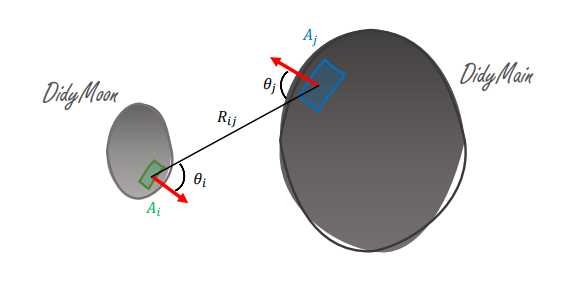
\includegraphics[width=.4\linewidth]{rsc/viewfac1.png} 
    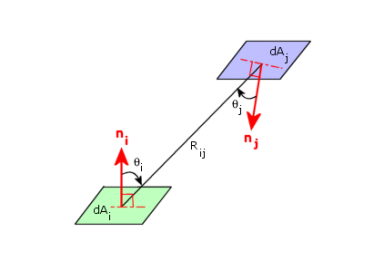
\includegraphics[width=.4\linewidth]{rsc/viewfac2.png}
    \captionof{figure}{(a) View factor on Didymos system and (b) View factor schematic interpretation}
\end{center}

Thus, this factor can be expressed as :
\begin{equation}
    V_{ij}=\frac{a_i cos \theta _i cos \theta _j}{\pi r^2}.
    \label{eq 43}
\end{equation}

$a_i$ is the surface area of element i (In our model, we consider $a_i=1$), $r$ is the distance between facets $i$ and $j$, and the angles $\theta$ are the angles between the facet outward normal and the line between facet centers. Using this factor, all facets with $\theta _i$ or $\theta _j$ $\geq 90 \deg $ are equals to 0 as they are not facing each other. \\

Considering now the direct thermal heating $u_{p,j}$ which is the largest flux from the primary due to the low albedo, we can write it as follow :
\begin{equation}
    u_{p,j}=\sum_{i \neq j}^N V_{ij} \epsilon \sigma u^4_{s,j}.
    \label{eq 44}
\end{equation}

Here, $T_{s,j}$ is the surface temperature of facet $j$.

In order to reduce computing time, temperatures of the primary are not computed, all facet temperatures $u_{s,j}$ from Eq. (\ref{eq 44}) are set to the same high value based on midday temperatures of the moon.In applying Eqs. (\ref{eq 44}) and (\ref{eq 42}) therefore an upper limit is derived for the occurring fluxes $W_p$ and $u_p$. The temperature change due to heating from the primary is evaluated by applying Eq. (5) which for the night side and the eclipse periods of the moon reduces to :
\begin{equation}
    W_p + u_p = \epsilon \sigma u^4 + \kappa \frac{du}{dx},
    \label{eq 45}
\end{equation}

Indeed, in addition to mutual heating implementation, we added the primary occultation on didymoon.

Using spice and \textit{cspice\_occult} function, we can determine if the moon is fully or partially in the shade of the primary body. During those phases, the algorithm avoid any direct solar flux and only compute mutual heating from the primary as shown in Eq. (\ref{eq 45})

\begin{center}
    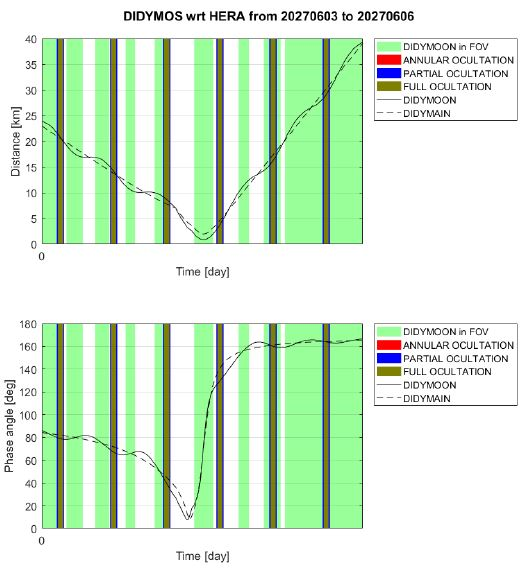
\includegraphics[scale=0.55]{rsc/occult.jpg}
    \captionof{figure}{FOV, Phase angle and Occultation Considerations (Green means Didymoon is fully visible by HERA)}
\end{center}

\subsection{Integration}

Using the Eq. (\ref{eq 41}), we implement the mutual heating to the current thermophysical model Eq. (1).\\

In order to check the result's consistency, several test has been performed in all possible configurations. As the algorithm takes every single facets of both primary and secondary bodies, we compute only the temperature for a single position at the equator.\\

The first test was performed using only the direct and indirect thermal from the primary, considering $Q_{Sun}=0$ for a long time period, thus the temperature could converge. This test doesn't have physical meanings as the direct flux from the Sun cannot be null for a such a time period but was performed to see the influence of the mutual heating and check if this one create a significant thermal flux.\\

\textbf{[TEST RESULTS WITH AND W/O QSUN]}\\

We also performed several tests taking positions all around the equator, in the shade and in the normal axis to the Sun and everything was consistent.\\

Then, after a full integration and with the exact same parameters, we compute the difference between simulations including mutual heating and not including it.\\

Thus, we have the following result :\\

\textbf{[DIFFERENCE BETWEEN WITH AND W/O MUTUAL HEATING]}
